%!TEX root = ../../../adrien_gomar_phd.tex

\subsection{Geometry}
\label{sub:cror_propeller_geometry}

A propeller is composed of a hub and a rotating set of 
$B$ blades as schematically represented in
Fig.~\ref{fig:cror_propeller_geometry}. The hub
is the part on which the blades are mounted.
We set the diameter of these blades being $D$
and their rotation speed being $\Omega$. 
In front of the propeller, there is a spinner which is
a conic geometry element that conducts the 
inflow to the propeller blades.
The propeller can be seen as
a turbofan whose fan is not within a nacelle.
\begin{figure}[htp]
  \centering
  \includegraphics*[scale=0.30]{propeller_geometry.pdf}
  \caption{Geometry of a propeller.}
  \label{fig:cror_propeller_geometry}
\end{figure}
Its absence implies that theoretically, the mass-flow can be
infinite. To quantify this, it is common for engines to
consider the bypass ratio. It is defined as the ratio of the
cold air (the fan exhaust)
divided by the hot air (the air that goes through the engine core).
To give an idea, one of the highest bypass ratio engine on today's aircraft is obtained
by the Pratt~\&~Whitney~PW1000G with a~12 bypass ratio. 
This number is representative of the mass-flow rate generated by the engine.
However, we have seen that mass-flow is a parameter that can be used to increase
the thrust so as the velocity difference. Assuming that in a classical ducted turbofan, 
the bypass ratio is limited to~12, the only
way to increase the thrust is to increase the 
velocity which deteriorates the propulsive efficiency.
For the sake of comparison, 
propellers are estimated to have a bypass ratio of~50. 
This explains why this architecture has
regained interest. However, propellers
have been limited to low Mach number flight condition
due to the high relative velocity seen at the tip of the blades
needed to achieve a high level of thrust.

\subsection{Velocity triangle}
\label{sub:cror_propeller_velocity_triangle}
The velocity triangle applied to a propeller configuration
is shown in Fig.~\ref{fig:cror_velocity_triangle_propeller}.
The aim of a propeller is to create thrust through an increase
of the axial velocity noted $\Delta V_x$ in the diagram. To do
so, the relative flow field is straighten up. This gives both
an increase in axial velocity but also in tangential velocity.
In fact, the inflow that was purely axial retrieves a tangential
component at the outlet. This is called the swirl and
is a lost energy as it cannot be used to produce thrust.
\begin{figure}[htp]
  \centering
  \includegraphics*[scale=0.40]{velocity_triangle_propeller.pdf}
  \caption{Velocity triangle applied to a propeller.}
  \label{fig:cror_velocity_triangle_propeller}
\end{figure}
Moreover, the relative velocity $W$ should be kept subsonic
otherwise the propulsive efficiency is reduced. This limits
the free-stream velocity $V_0$ of the aircraft and the size of 
the propeller as the rotation speed velocity depends on
the radius of the blades.

\subsection{Similarity coefficients}
\label{sub:similarity_coefficients}
To evaluate the performance of the propeller, four similarity
coefficients are commonly used:
the advance ratio $J$ that represents the operating point of the propeller,
the thrust $C_t$ and power $C_p$ coefficients and finally
the efficiency $\eta$
\begin{equation}
    J = \frac{V_0}{n D}, \quad
    C_T = \frac{F_x}{\rho n ^ 2  D ^ 4}, \quad
    C_P = \frac{M_x \Omega}{\rho n ^ 3 D ^ 5}, \quad
    \eta = J \frac{C_T}{C_P},
\end{equation}
where $V_0$ is the free-stream velocity 
as shown in Fig.~\ref{fig:cror_propeller_geometry},
$\rho$ the free-stream density,
$n$ the rotation frequency ($n = \Omega / 2 \pi$) and
$M_x$ the axial torque.
The efficiency defined here is the global propulsive efficiency
as it gives the ratio of the propulsive power over the mechanical power.

An estimation of the variation of the advance ratio $J$ and the 
efficiency $\eta$ depending on the flight conditions can be given as follow~\cite{Bousquet2012}
\begin{alignat}{4}
    \text{(cruise)} \quad  0.8 &< \eta &< 0.95, \quad 1 &< J < 3.5 \\
    \text{(take-off and landing)} \quad  0.5 &< \eta &< 0.8, \quad J &< 1.
    \label{eq:estimation_sim_coeff}
\end{alignat}

\subsection{Main physical phenomena}
\label{sub:cror_propeller_physics}

\begin{figure}[htp]
  \centering
  \subfigure[wakes]{
      \label{fig:propeller_wakes}
      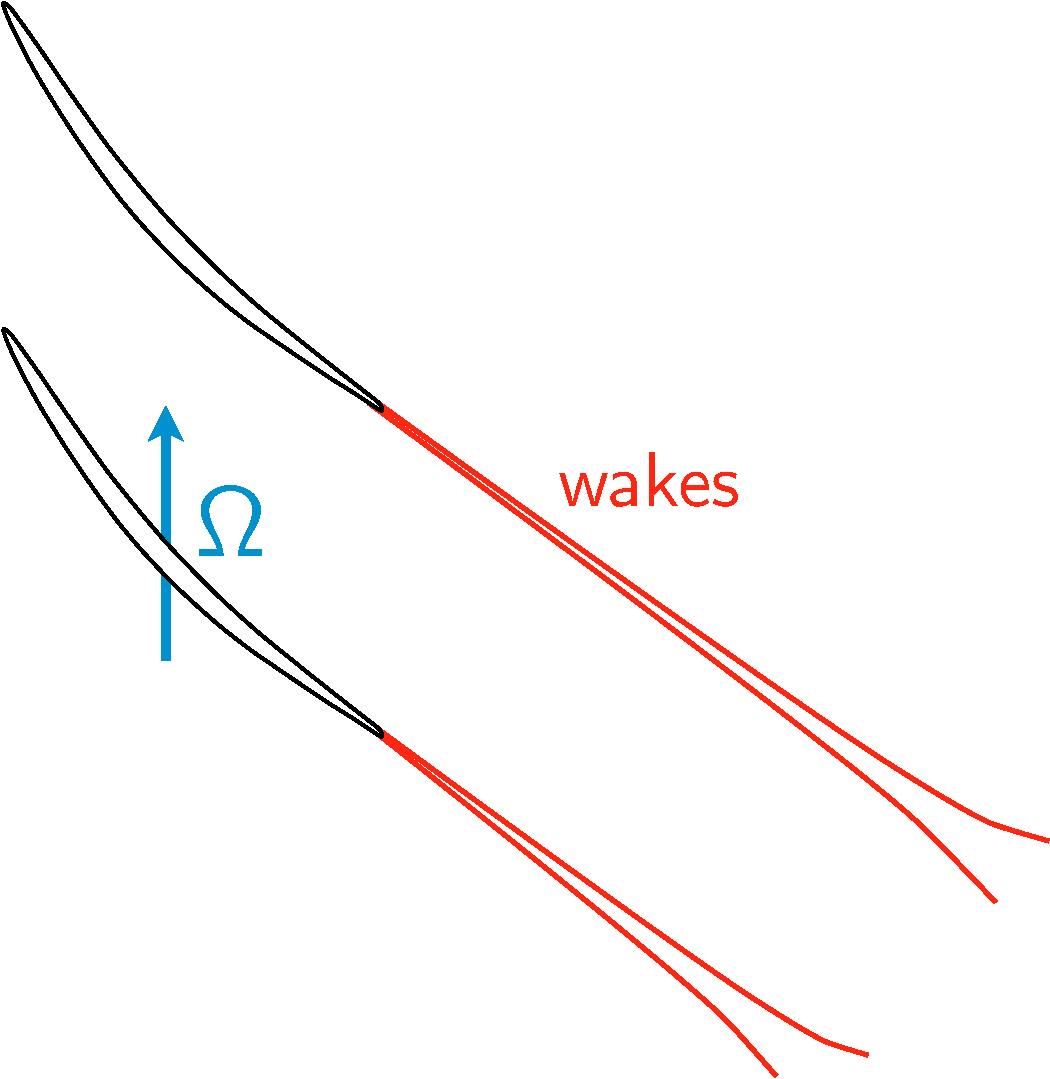
\includegraphics[scale=.2]{propeller_wakes.pdf}}
  \quad\subfigure[tip vortices]{
      \label{fig:propeller_tip_vortices}
      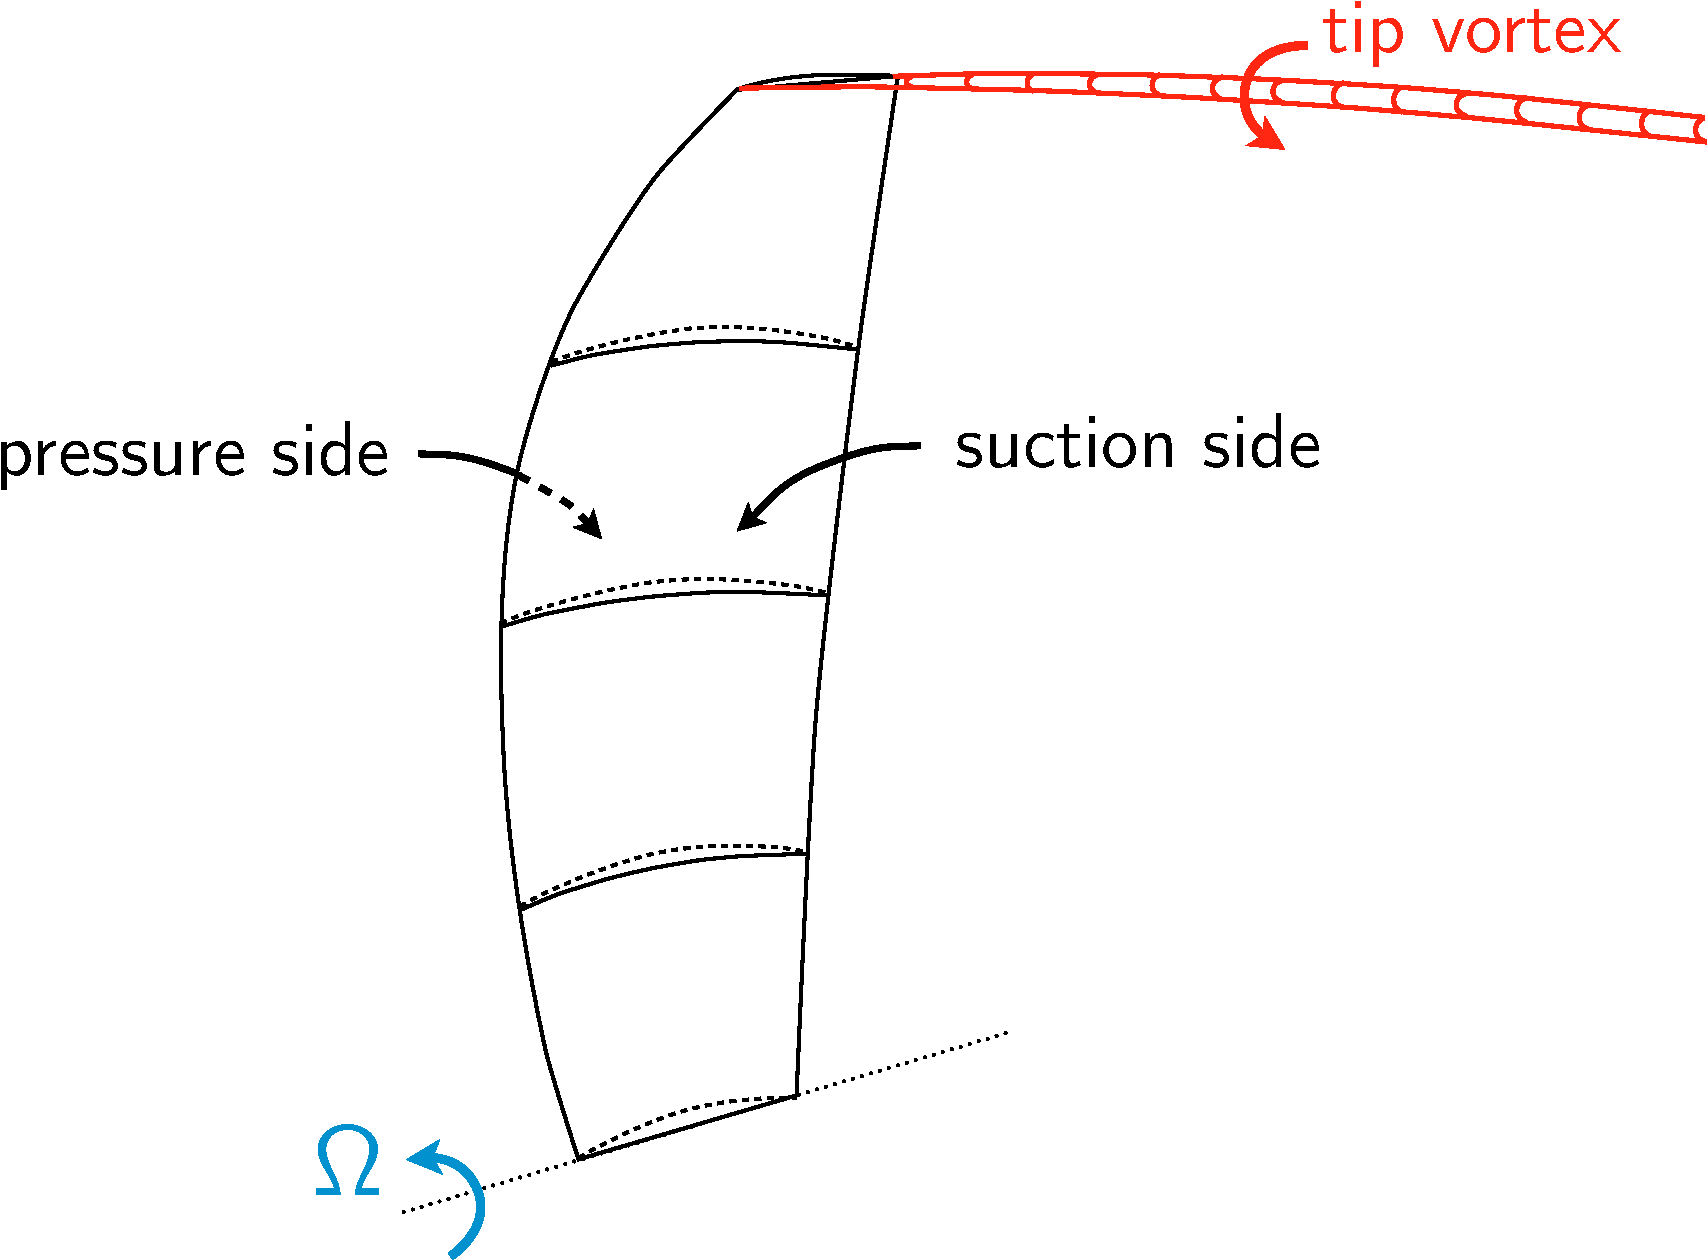
\includegraphics[scale=.2]{propeller_tip_vortices.pdf}}
  \quad\subfigure[stream tube contraction]{
      \label{fig:propeller_stream_tube}
      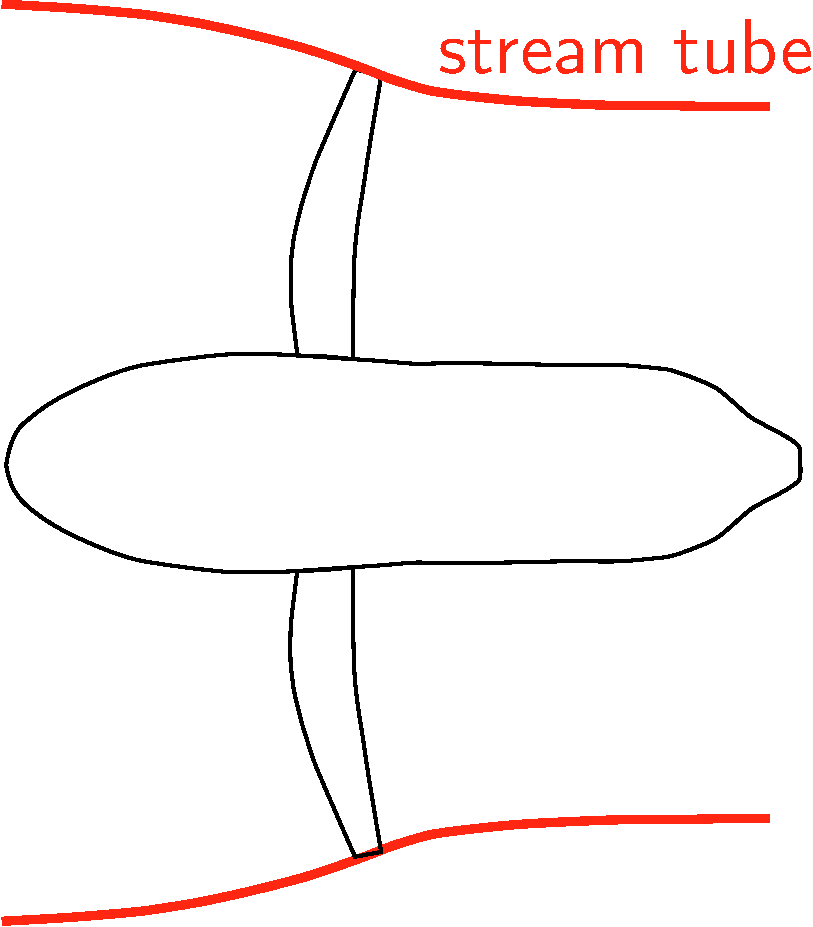
\includegraphics[scale=.2]{propeller_stream_tube.pdf}}
  \caption{Main physical phenomena seen in a propeller.}
  \label{fig:propeller_phys_phenomena}
\end{figure}
The main physical phenomena that can be seen in a propeller are schematically represented
in Fig.~\ref{fig:propeller_phys_phenomena}. Firstly, due to the presence of a boundary
layer on the pressure side and suction side of the blades, a wake is shed behind each blade, which
is represented by a momentum deficit (Fig.~\ref{fig:propeller_wakes}). 
It is mostly a two-dimensional
phenomenon seen at each radius. Secondly, 
in the tip region of the blade, the pressure difference between each 
side of the blade induces a vortex that is counter-rotating with respect to 
the rotation speed (Fig.~\ref{fig:propeller_tip_vortices}). 
They are advected by the local relative velocity giving them
an helical path propagating downstream.
To reduce this phenomenon, one way is to modify the geometry of the tip
of the blades.
Finally, the propeller generates thrust through an acceleration of the fluid. Thus, the stream
tube is contracted (Fig.~\ref{fig:propeller_stream_tube}). 
All of these phenomena are stationary in their relative frame of reference.
